\subsection{Erros de gradiente de campo}\label{sec:2.11}
Agora, pode-se analisar os efeitos dos erros de gradiente nas oscilações betatron em torno da órbita ideal. Estes "erros" são relativos aos desvios da função de focalização $K(s)$ do seu valor nominal em cada coordenada $s$. Pode-se escrever
\begin{align*}
	K(s)_{atual} = K(s)_{nominal} + k(s)
\end{align*}
onde assume-se que $k(s)$ é pequeno. O efeito do desvio $k(s)$ será mudar a função betatron do seu valor nominal $\beta(s)$ para um novo valor $\beta(s)+\Delta \beta(s)$. Desta forma, a sintonia também será alterada do seu valor nominal $\nu$ para um novo valor $\nu + \Delta \nu$. Geralmente, a mudança de sintonia $\Delta \nu$ é mais preocupante, uma vez que esta pequena mudança pode fazer com que o ponto de operação da máquina entre em uma ressonância.

Suponha que existe um erro de gradiente $k$ apenas em um pequeno intervalo $\Delta s$ em $s=0$. Então um elétron que passa em $s=0$ irá receber um \textit{kick} angular extra $\Delta x'$ proporcional ao seu desvio $x$. Isto é,
\begin{align}
	\Delta x' = -k\ \Delta s\ x\label{eq:2.96}
\end{align}

\begin{proof}
	Fazendo um raciocínio bem informal, sabe-se que a equação diferencial que descreve o movimento do elétron é
	\begin{align*}
		x'' = -K(s)x
	\end{align*}
	A derivada nada mais é que a variação de $x'$ em um intervalo $s$ pequeno, então $x'' = \Delta x'/\Delta s$. Logo,
	\begin{align*}
		\frac{\Delta x'}{\Delta s} &= -K(s)x\\
		\Delta x' &= -K(s)x \Delta s
	\end{align*}
	Analisando apenas a variação de $x'$ causada pela variação $k(s)$ da função de focalização, tem-se
	\begin{align*}
		\Delta x' &= -k\ \Delta s\ x
	\end{align*}
\end{proof}

Aproximando novamente a função betatron por uma simples oscilação harmônica, o que aconteceria se um elétron chegasse em $s=0$ no pico da oscilação? O movimento seria como a curva representada na \autoref{fig:fig23}.

\begin{figure}[!htb]
	\centering
	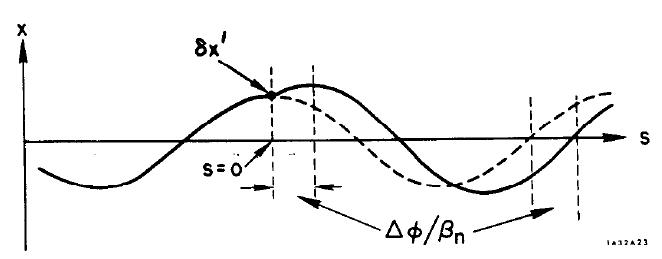
\includegraphics[width=0.7\linewidth]{./Figuras/fig23.jpeg}
	\caption{Efeito do gradiente de erro em $s=0$. Retirado de \cite{sands1970physics}.}
	\label{fig:fig23}
\end{figure}

Antes de chegar em $s=0$, o desvio era dado por
\begin{align}
	x = b\ cos(s/\beta_n)
\end{align}
e, depois de $s=0$, seguirá uma trajetória
\begin{align}
	x = (b+\Delta b)cos(s/\beta_n + \Delta \varphi)
\end{align}
onde
\begin{align}
	-\frac{b+\Delta b}{\beta_n}\ sen(\Delta \varphi) = \Delta x'
\end{align}

\begin{proof}
	Seja a solução da equação diferencial $x'' = -Kx$ dada por $x = a\ cos(\varphi-\vartheta)$. Para $K(s) = K(s)_{nominal}$ já foi visto que existe a solução aproximada $x = b\ cos(s/\beta_n)$. Quando o elétron passa em $s=0$, a equação diferencial deixa de ser $x'' = -K(s)_{nominal}\ x$ e passa a ser $x'' = -K(s)_{atual}\ x$ onde $K(s)_{atual} = K(s)_{nominal} + k(s)$. Logo, a equação diferencial é dada por $x'' = -(K(s)_{nominal} + k(s))x$. Esta mudança na função de focalização $K(s)$ acarretará numa mudança $\Delta \beta$ no valor da função betatron. Como tanto a amplitude quanto a fase de oscilação dependem de $\beta(s)$, ambas sofreram alterações, as quais foram denominadas $\Delta b$ e $\Delta \varphi$, respectivamente. Sendo assim, a solução desta nova equação diferencial pode ser escrita como
	\begin{align*}
		x = (b+\Delta b)\ cos(s/\beta_n + \Delta \varphi)
	\end{align*}
	Nota-se que o termo $\Delta \varphi$ não está multiplicado pela variável $s$ como o termo $1/\beta_n$. Isto porque a alteração na fase da oscilação ocorre somente no ponto $s=0$, diferentemente do avanço de fase descrito pelo termo $s/\beta_n$.
	
	Agora, derivando a expressão $x = b\ cos(s/\beta_n)$, tem-se
	\begin{align*}
		x' &= -\frac{b}{\beta_n}\ sen(s/\beta_n)\\
		\therefore x'(0) &= 0 = x'_i
	\end{align*}
	Derivando a expressão $x = (b+\Delta b)\ cos(s/\beta_n + \Delta \varphi)$, tem-se
	\begin{align*}
		x' = -\frac{b+\Delta b}{\beta_n}\ sen(s/\beta_n + \Delta \varphi)\\
		x'(0) = -\frac{b+\Delta b}{\beta_n}\ sen(\Delta \varphi) = x'_f
	\end{align*}
	Desta forma, a variação $\Delta x'$ da inclinação do movimento no ponto $s=0$ é
	\begin{align*}
		\Delta x' &= x'_f - x'_i\\
				  &= -\frac{b+\Delta b}{\beta_n}\ sen(\Delta \varphi) - 0\\
				  & = -\frac{b+\Delta b}{\beta_n}\ sen(\Delta \varphi)
	\end{align*}
	c.q.d.
\end{proof}

Para pequenos valores de $\Delta x'$, $\Delta \varphi$ é pequeno (ou seja, pode-se aproximar $sen(\varphi) = \varphi$) e $\Delta b$ é muito menor que $b$. Logo,
\begin{align}
	\Delta \varphi \approx -\frac{\beta_n\ \Delta x'}{b}
\end{align}
Utilizando a equação \eqref{eq:2.96} -- e lembrando que em $s=0$ o deslocamento é $b$ -- tem-se que
\begin{align*}
	\Delta \varphi = \beta_n\ k\ \Delta s
\end{align*}
O efeito do erro de gradiente é basicamente alterar a fase de oscilação por $\Delta \varphi$. Agora, lembre-se que $2\pi\nu$ é o avanço de fase total em uma revolução; então, grosseiramente falando, o erro de gradiente acarreta em
\begin{align}
	\Delta \nu \approx - \frac{\Delta \varphi}{2\pi} = -\frac{\beta_n\ k\ \Delta s}{2\pi}
\end{align}
O sinal negativo vem do fato de que o avanço total de fase é reduzido.

Este resultado é, na verdade, até duas vezes maior do que o normal. O motivo é que o cálculo de $\Delta \varphi$ foi feito no caso especial do elétron chegando em $s=0$ no pico da oscilação. Se o elétron chegar em $s=0$ com uma fase $\varphi_0$, a mudança de fase $\Delta \varphi$ é reduzida por um fator $cos^2(\varphi_0)$. Como $\varphi_0$ assume vários valores ao longo de sucessivas voltas, pode-se esperar que a média de $\Delta \varphi$ seja reduzida pela média de $cos^2(\varphi_0)$, que é apenas $1/2$. Com esta correção, a estimativa de $\Delta \nu$ fica
\begin{align}
	\Delta \nu = -\frac{1}{4\pi}\beta(s)\ k\ \Delta s
\end{align}

\begin{proof}
	Seguindo o mesmo raciocínio da demonstração anterior -- porém considerando um elétron que chega em $s=0$ com uma fase $\varphi_0$ -- tem-se que o movimento do elétron antes do \textit{kick} é dado por $x = b\ cos(s/\beta_n + \varphi_0)$. Logo,
	\begin{align*}
		x' &= -\frac{b}{\beta_n}\ sen(s/\beta_n + \varphi_0)\\
		\therefore x'(0) &= -\frac{b}{\beta_n}\ sen(\varphi_0) = x'_i
	\end{align*}
	Depois do \textit{kick}, o movimento do elétron é dado pela expressão $x = (b+\Delta b)\ cos(s/\beta_n + \Delta \varphi + \varphi_0)$. Derivando-a,
	\begin{align*}
		x' = -\frac{b+\Delta b}{\beta_n}\ sen(s/\beta_n + \Delta \varphi + \varphi_0)\\
		x'(0) = -\frac{b+\Delta b}{\beta_n}\ sen(\Delta \varphi + \varphi_0) = x'_f
	\end{align*}
	Desta forma, a variação $\Delta x'$ da inclinação do movimento no ponto $s=0$ é
	\begin{align*}
		\Delta x' &= x'_f - x'_i\\
				  &= -\frac{b+\Delta b}{\beta_n}\ sen(\Delta \varphi + \varphi_0) + \frac{b}{\beta_n}\ sen(\varphi_0)
	\end{align*}
	Por trigonometria, $sen(\Delta \varphi + \varphi_0) = sen(\Delta \varphi)cos(\varphi_0) + cos(\Delta \varphi)sen(\varphi_0)$. Substituindo:
	\begin{align*}
		\Delta x' &= -\frac{b+\Delta b}{\beta_n}\ [sen(\Delta \varphi)cos(\varphi_0) + cos(\Delta \varphi)sen(\varphi_0)] + \frac{b}{\beta_n}\ sen(\varphi_0)
	\end{align*}
	Como $\Delta \varphi$ é pequeno, pode-se aproximar $sen(\Delta \varphi) \approx \Delta \varphi$ e $cos(\Delta \varphi) \approx 1$. Logo,
	\begin{align*}
		\Delta x' &= -\frac{b+\Delta b}{\beta_n}\ [\Delta \varphi\ cos(\varphi_0) + sen(\varphi_0)] + \frac{b}{\beta_n}\ sen(\varphi_0)\\
				  &= -\frac{b+\Delta b}{\beta_n}\ \Delta \varphi\ cos(\varphi_0) - \frac{\Delta b}{\beta_n}\ sen(\varphi_0)
	\end{align*}
	Descartando o termo de segunda ordem,
	\begin{align*}
		\Delta x' &= -\frac{b}{\beta_n}\ \Delta \varphi\ cos(\varphi_0) - \frac{\Delta b}{\beta_n}\ sen(\varphi_0)
	\end{align*}
	Agora, pela continuidade do movimento do elétron, tem-se que
	\begin{align*}
		b\ cos(\varphi_0) = (b+\Delta b)\ cos(\Delta \varphi + \varphi_0)
	\end{align*}
	Por trigonometria, $cos(\Delta \varphi + \varphi_0) = cos(\Delta \varphi)cos(\varphi_0) - sen(\Delta \varphi)sen(\varphi_0)$. Substituindo esta relação e novamente aproximando $sen(\Delta \varphi)$ e $cos(\Delta \varphi)$, tem-se
	\begin{align*}
		b\ cos(\varphi_0) = (b+\Delta b)[cos(\varphi_0)-\Delta \varphi\ sen(\varphi)]
	\end{align*}
	Manipulando a expressão, tem-se que
	\begin{align*}
		\frac{\Delta b}{(b+\Delta b)\Delta \varphi} = tg(\varphi_0)
	\end{align*}
	Descartando o termo de segunda ordem:
	\begin{align*}
		\frac{\Delta b}{b \Delta \varphi} &= tg(\varphi_0)\\
		\therefore \Delta b &= b\ \Delta \varphi\ tg(\varphi_0)
	\end{align*}
	Substituindo esta relação na expressão de $\Delta x'$, tem-se
	\begin{align*}
		\Delta x' &= -\frac{b}{\beta_n}\ \Delta \varphi\ cos(\varphi_0) - \frac{b\ \Delta \varphi\ tg(\varphi_0)}{\beta_n}\ sen(\varphi_0)\\
				  &= -\frac{b}{\beta_n}\ \Delta \varphi\ cos(\varphi_0) - \frac{b\ \Delta \varphi\ sen^2(\varphi_0)}{\beta_n\ cos(\varphi_0)}
	\end{align*}
	Multiplicando ambos os lados da equação por $cos(\varphi_0)$:
	\begin{align*}
		cos(\varphi_0)\ \Delta x' &= -\frac{b}{\beta_n}\ \Delta \varphi\ cos^2(\varphi_0) - \frac{b\ \Delta \varphi\ sen^2(\varphi_0)}{\beta_n}\\
			&= -\frac{b\ \Delta \varphi}{\beta_n}[cos^2(\varphi_0)+sen^2(\varphi_0)]\\
			&= -\frac{b\ \Delta \varphi}{\beta_n}
	\end{align*}
	Da equação \eqref{eq:2.96}, sabe-se que $\Delta x' = -k\ \Delta s\ x$. Logo,
	\begin{align*}
		-k\ \Delta s\ x\ cos(\varphi_0) &= -\frac{b\ \Delta \varphi}{\beta_n}
	\end{align*}
	Mas, pela aproximação feita, $x = b\ cos(s/\beta_n + \varphi_0)$. Logo, $x(0) = b\ cos(\varphi_0)$. Substituindo,
	\begin{align*}
		-k\ \Delta s\ b\ cos^2(\varphi_0) &= -\frac{b\ \Delta \varphi}{\beta_n}\\
		\therefore \Delta \varphi &= \beta_n\ k\ \Delta s\ cos^2(\varphi_0)
	\end{align*}
	Como já foi dito anteriormente,
	\begin{align*}
		\Delta \nu \approx - \frac{\Delta \varphi}{2\pi} = -\frac{\beta_n\ k\ \Delta s\ cos^2(\varphi_0)}{2\pi}
	\end{align*}
	Na média, $cos^2(\varphi_0) = 1/2$. Logo,
	\begin{align*}
		\Delta \nu = -\frac{1}{4\pi}\beta k \Delta s
	\end{align*}
	c.q.d.
\end{proof}

Note que a mudança da sintonia é proporcional ao erro de gradiente em qualquer ponto e ao valor de $\beta$ neste ponto. Novamente, pode-se observar que a função $\beta$ é um indicador da sensibilidade do anel a imperfeições.

Se existe um erro de gradiente $k(s)$ distribuído ao longo do anel, a alteração total da sintonia é
\begin{align}
	\Delta \nu = -\frac{1}{4\pi} \int\limits_{0}^{L}\beta(s)k(s)ds\label{eq:2.104}
\end{align}

Foi dito anteriormente que é esperado que $\Delta \nu$ seja da dimensão de $\nu$, então grandes valores de $\nu$ devem ser evitados. Para checar este fato, lembre (da \autoref{sec:2.10}) que $\beta$ é esperado para ser escalado como $|K|^{-1/2}$. Sendo assim, $\nu$ deve ter a mesma dimensão que $|K|^{1/2}$. Da equação \eqref{eq:2.104}, $\Delta \nu$ deve ser da magnitude de $k\beta$, então $\Delta \nu/\nu$ deve ser da mesma dimensão que $k/K$. Para um dado tamanho relativo do erro de gradiente, a alteração da sintonia $\Delta \nu$ é proporcional a $\nu$. Mas o espaço entre as ressonâncias é independente de $\nu$, então grandes valores de $\nu$ implicam em uma máquina mais delicada.

Uma mudança em $\nu$ implica que deve ter ocorrido uma mudança em $\beta$, a qual ainda não ficou muito evidente nos cálculos realizados. Pode-se mostrar que
\begin{align}
	\Delta \beta(s) = \frac{\beta(s)}{2\ sen(2\pi\nu)}\int\limits_{0}^{L}k(\bar{s})\ \beta(\bar{s})\ cos\ 2\{|\varphi(s)-\varphi(\bar{s})|-\pi\nu\}d\bar{s}\label{eq:2.105}
\end{align}
onde, como já é conhecido,
\begin{align}
	\varphi(s) = \int\limits_{0}^{s}\frac{d\bar{s}}{\beta(\bar{s})}
\end{align}

Pode-se comparar este resultado com o que foi obtido na equação \eqref{eq:2.94} para as distorções de órbita fechada. A forma é similar, mas com duas diferenças importantes. Primeiro, enquanto $\beta^{1/2}$ aparece na integral para os desvios da órbita fechada, $\beta$ aparece na integral para $\Delta \beta$. Segundo, note que o argumento do termo senoidal no denominador é $2\pi\nu$ ao invés de $\pi\nu$. A "explosão" ressonante ocorre tanto nos valores inteiros quanto nos meio inteiros de $\nu$. O erro de gradiente introduz um novo grupo de ressonâncias no diagrama de operação de $\nu_x$ po $\nu_z$, as quais devem ser evitadas em um anel de armazenamento em operação.

A mudança de sintonia $\Delta \nu$ vem, claro, da mudança na função betatron. Da definição de $\nu$, pode-se escrever
\begin{align}
	2\pi\nu = \int\limits_{0}^{L}\frac{\Delta \beta(s)}{\beta^2(s)}ds
\end{align}
Uma integração em $s$ de $\Delta \beta(s)/\beta^2(s)$ utilizando a equação \eqref{eq:2.105} chega no mesmo resultado para $\Delta \nu$ obtido na equação \eqref{eq:2.104}.

Neste ponto, pode-se esperar um certo questionamento: por que $\Delta \beta$ tem uma explosão ressonante em valores meio inteiros de $\nu$ e a mudança de sintonia $\Delta \nu$ não? A razão para este fato é que a expressão derivada para $\Delta \nu$ é válida apenas para pequenas variações de $\beta$, o que não acontece em ressonâncias, nas quais $\beta$ diverge. Um cálculo mais preciso deve ser feito, mantendo os efeitos de segunda ordem causados pela perturbação $k$, para encontrar $\Delta \nu$ -- e, de fato, o próprio $\Delta \beta$ -- próximo a uma ressonância.